%Grundlagen\\
%- äußere Schalenelektronen für gewöhnlich nach Boltzmann (thermisch) verteilt\\
%- optisches Pumpen sorgt für nicht-thermische Verteilung\\
%
Ein Atom hat diskrete Energieniveaus, auf denen sich die Hüllenelektronen befinden.
Die Verteilung der Elektronen erfolgt bei den äußeren Hüllenelektronen statistisch nach Boltzmann.
Die Besetzungszahlen $N_{1}, N_{2}$ zweier Niveaus mit der statistischen Gewichtung $g_{1}, g_{2}$ liegen in folgendem Zusammenhang:
\begin{equation*}
  \frac{N_{2}}{N_{1}} = \frac{ g_{2} \exp{  \left( -\frac{W_{2}}{k_{\text{B}}}  \right) }}{ g_{1} \exp{ \left( -\frac{W_{1}}{k_{\text{B}}} \right) }}.
\end{equation*}
Das Prinzip des optischen Pumpens besetzt die Niveaus entgegen dieser thermischen Verteilung.\\
%
%Landé-Faktor\\
%- Materialeigenschaft -> Materialbestimmung über diese Messung möglich\\
%- Verhältnisfaktor für das magnetische Moment von Spin, Bahndrehimpuls, etc. zum Bohrschen Magneton\\
%- Bohrsches Magneton: magnetisches Moment für Elektron mit l=1????\\
%- Herleitung: Winkelbeziehungen etc\\
%
Der Landé-Faktor $g$ ist eine Materialeigenschaft, die zur Stoff- und Isotopenbestimmung benutzt werden kann.
Das Bohr'sche Magneton ist der Betrag des magnetischem Momentes $\vec{\mu}$ eines Elektrons mit Bahndrehimpuls $L=1$.
Der Landé-Faktor ist ein Verhältnisfaktor für die magnetischen Momente des Spins $\vec{S}$, des Bahndrehimpulses $\vec{L}$, des Gesamtdrehimpulses $\vec{J}$, etc. zum Bohr'schen Magneton $\mu_{\text{B}}$:
Das magnetische Moment zu dem Spin $\vec{S}$ sieht wie folgt aus:
\begin{align*}
  \vec{\mu_{\text{S}}} = - g_{\text{S}} \mu_{\text{B}} \vec{S} && \text{mit} && |\vec{\mu_{\text{S}}}|= g_{\text{S}} \mu_{\text{B}} \sqrt{S(S+1)}.\\
\end{align*}
Entsprechend ist das magnetische Moment des Bahndrehimpuls $\vec{L}$
\begin{align*}
  \vec{\mu_{\text{L}}} = - \mu_{\text{B}} \vec{L} && \text{mit} && |\vec{\mu_{\text{L}}}|= \mu_{\text{B}} \sqrt{L(L+1)}.
\end{align*}
\begin{figure}[h!]
  \centering
  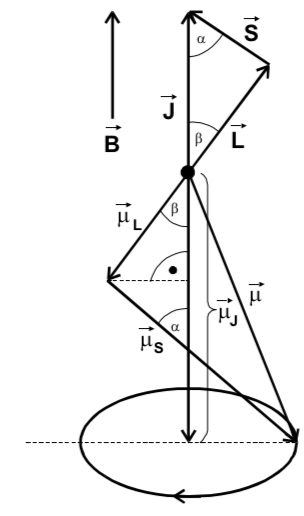
\includegraphics[width=0.3\textwidth]{magmom1.png}
  \caption{Darstellung der verschiedenen magnetischen Momente von Spin, Bahndrehimpuls und Gesamtdrehimpuls \cite{1}}
  \label{fig:magmom}
\end{figure}
Die Kopplung von Spin und Bahndrehimpuls ergibt den Gesamtdrehimpuls $\vec{J}$ und das zugehörige magnetische Moment $\vec{\mu_{\text{J}}}$:
\begin{align*}
  \vec{\mu_{\text{J}}} = \vec{\mu_{\text{S}}} + \vec{\mu_{\text{L}}}= - g_{\text{J}} \mu_{\text{B}} \vec{J} && \text{mit} && |\vec{\mu_{\text{J}}}|=  g_{\text{J}} \mu_{\text{B}} \sqrt{J(J+1)}.
\end{align*}
Nur das magnetische Moment $|\vec{\mu_{\text{J}}}|$ in Richtung von $\vec{J}$ hat schlussendlich einen Effekt, da $\vec{J}$ eine Präzessionsbewegung vollführt (Abb. \ref{fig:magmom}).
Die Winkelbeziehung in $|\vec{\mu_{\text{J}}}|$ lässt sich aus Abbildung \ref{fig:magmom} erkennen.
Damit ergibt sich:
\begin{align*}
                  && |\vec{\mu_{\text{J}}}|  &=&  |\mu_{\text{S}}| \cos{(\alpha)} &+& |\mu_{\text{L}}| \cos{(\beta)} \\
 \Leftrightarrow  && g_{\text{J}} \mu_{\text{B}} \sqrt{J(J+1)} &=& g_{\text{S}} \mu_{\text{B}} \sqrt{S(S+1)} \cos{(\alpha)} &+& \mu_{\text{B}} \sqrt{L(L+1)} \cos{(\beta)}
\end{align*}
Für die Winkel lässt sich aufstellen:
\begin{align*}
  \cos{(\alpha)} &=& \frac{ |\vec{S}|^2 - |\vec{L}|^2 + |\vec{J}|^2}{2 |\vec{L}||\vec{J}|^2} \\% &=& \frac{ \left(g_{\text{S}} \mu_{\text{B}} \sqrt{S(S+1)}\right)^2  -  \left( \mu_{\text{B}} \sqrt{L(L+1)} \right)^2  +  \left( g_{\text{J}} \mu_{\text{B}} \sqrt{J(J+1)} \right)^2 }{  2              \mu_{\text{B}} \sqrt{L(L+1)} g_{\text{J}} \mu_{\text{B}} \sqrt{J(J+1)}    } \\
  \cos{(\beta)}  &=& \frac{-|\vec{S}|^2 + |\vec{L}|^2 + |\vec{J}|^2}{2 |\vec{S}||\vec{J}|^2}.\\% &=& \frac{-\left(g_{\text{S}} \mu_{\text{B}} \sqrt{S(S+1)}\right)^2  +  \left( \mu_{\text{B}} \sqrt{L(L+1)} \right)^2  +  \left( g_{\text{J}} \mu_{\text{B}} \sqrt{J(J+1)} \right)^2 }{  2 g_{\text{S}} \mu_{\text{B}} \sqrt{S(S+1)} g_{\text{J}} \mu_{\text{B}} \sqrt{J(J+1)}    }.\\
\end{align*}
Schlussendlich ergibt sich:
\begin{equation}
  g_{\text{J}}= \frac{\left(g_{\text{S}} +1 \right)J\left(J+1\right) + \left(g_{\text{S}}-1\right) \left[ S\left(S+1\right)-L\left(L-1\right) \right]   }{2J\left(J+1\right)}.
\label{eqn:landej}
\end{equation}
%
%Zeeman-Effekt\\
%- Aufspaltung der Hyperfeinstruktur durch ein äußeres Magnetfeld\\
%- Aufspaltung proportional zum Landé-Faktor\\
%
Der Zeemaneffekt beschreibt die Aufspaltung der vorhandenen Energieniveaus durch ein äußeres Magnetfeld.
Die magnetischen Momente wechselwirken mit dem äußeren Magnetfeld $\vec{B}$ und es haben nur die Beiträge entlang der $\vec{J}$-Achse einen Effekt.
Durch die Richtungsquantelung ist die Wechselwirkungsenergie $E_{\text{mag}}$ ein ganzzahliges Vielfaches $M_{\text{J}}$ von $g_{\text{J}} \mu_{\text{B}} B$:
\begin{equation}
  E_{\text{Zeeman}} = -\vec{\mu_{\text{J}}} \vec{B} \Leftarrow E_{\text{Zeeman}} = M_{\text{J}} g_{\text{J}} \mu_{\text{B}} B.
  \label{eqn:zeeman}
\end{equation}
%
%Kernspin\\
%- Eigendrehimpuls des Atomkerns\\
%- neuer Landé-Faktor\\
%\begin{equation}
%  g_{\text{F}}= g_{\text{J}} \frac{ F\left(F+1\right) + J\left(J+1\right) - I\left(I-1\right)  }{2 \sqrt{F\left(F+1\right)}}
%\label{eqn:landef}
%\end{equation}
%
Der Kernspin $\vec{I}$ entspricht dem Eigendrehimpuls des Atomkerns und führt zur Aufspaltung der Energieniveaus im Rahmen der Hyperfeinstruktur.
Die Hyperfeinstruktur wird durch den Zeemaneffekt weiter aufgespalten (Abb. \ref{fig:kernspin}).
\begin{figure}[h!]
  \centering
  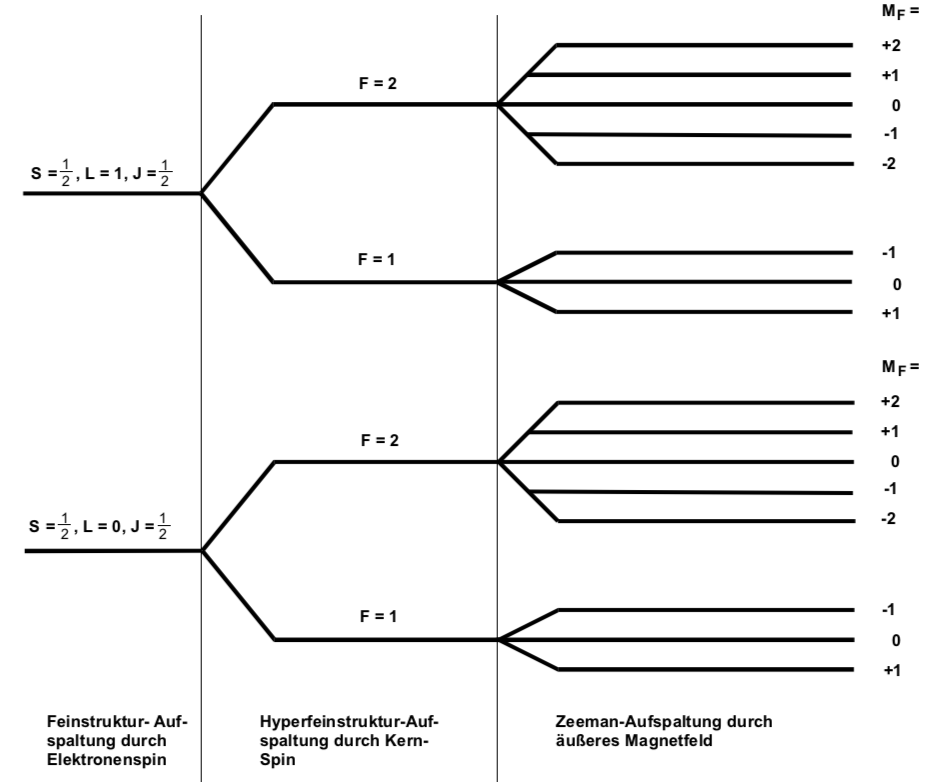
\includegraphics[width=\textwidth]{kernspin1.png}
  \caption{Darstellung der Aufspaltung der Energieniveaus durch die Hyperfeinstruktur und den Zeemaneffekt \cite{1}}
  \label{fig:kernspin}
\end{figure}
Der Gesamtdrehimpuls $\vec{J}$ des Elektrons und der Kernspin $\vec{I}$ koppeln zu dem Gesamtdrehimpuls $\vec{F}$ des Atoms:
\begin{align*}
  \vec{F}=\vec{J}+\vec{I} && mit && |\vec{\mu_{\text{F}}}|= g_{\text{F}} \mu_{\text{B}} \sqrt{F(F+1)}.\\
\end{align*}
Der Kernspin beeinflusst auch den Landé-Faktor $g_{\text{F}}$, der sich nun wie folgt berechnet:
\begin{equation}
  \mu_{\text{F}}= g_{\text{F}} \mu_{\text{B}} \frac{F(F+1) + J(J+1) - I(I+1)}{2 \sqrt{F(F+1)}}
  \label{eqn:landef}
\end{equation}
%
%Idee des optischen Pumpens\\
%- Übergänge der Elektronen auf den Energieniveaus durch Anregung\\
%- um bestimmte Übergänge zu produzieren, bestimmtes Spektrallicht einstrahlen ($D_{1}$-Licht)\\
%  --- Anregung/Quantensprünge $E_{2}-E_{1}=h \nu$\\
%- um GANZ bestimmte Übergänge zu produzieren, bestimmtes polarisiertes Licht einstrahlen ($\sigma^{+}$-Licht)\\
%  ——- Auswahlregeln\\
%- angeregte Zustände fallen in alle Grundzustände zurück\\
%- $\sigma^{+}$ pumpt (über die genannten Umwege) die Elektronen aus dem niedrigerem Grundzustand in den höheren Grundzustand\\
%








Optisches Pumpen + Aufbau\\
- zunächst sind alle Anregungen möglich, da die Elektronen noch auf allen Niveaus vorhanden sind\\
- das Licht wird also vollständig absorbiert\\
- mit der Zeit werden die Elektronen in einem Energieniveau gesammelt\\
- es sind keine Absorptionen möglich\\
- das Gas wird zunehmend transparent\\

Emission\\
- spontane Emission: Elektron fällt von alleine zurück (statistisch)\\
  --- Wahrscheinlich bei hohen Frequenzen des RF-Felds\\
- induzierte Emission: Elektron fällt zurück entlang der Energie der eingestrahlten Photonen (RF-Quanten)\\
  --- Wahrscheinlich bei niedrigen Frequenzen des RF-Felds\\
- induzierte Emission bei 'Resonanzstelle' (passendes RF-Feld mit der richtigen Energie für induzierte Emission)\\
\begin{equation}
  h \nu = g_{\text{J}} \mu_{\text{B}} \Delta M_{\text{J}} B_{\text{m}} \Leftrightarrow B_{\text{m}} = \frac{4 \pi m_{0}}{e_{0} g_{\text{J}}} \nu
\label{eqn:resonanz}
\end{equation}

Optisches Pumpen + Kernspin\\
- Energie der Spektrallinie überdeckt alle Hyperfeinstrukturen und Zeemaneffekt\\
- $\sigma^{+}$-Licht lässt nur $\Delta M_{\text{F}}= +1$ zu, also sammeln sich die Elektronen bei $^{2}S_{1/2}, F=2, M_{\text{F}}=+2$ \\

Quadratischer Zeemaneffekt/Breit-Rabi-Formel\\
- große B-Felder\\
- Wechselwirkung Spin-Bahn-Kopplung\\
- Wechselwirkung magnetische Momente\\
\begin{equation}
U_{\text{HF}}= g_{\text{F}} \mu_{\text{B}} B + g_{\text{F}}^2 \mu_{\text{B}}^2 B^2 \frac{(1- 2M_{\text{F}})}{\Delta E_{\text{HF}}}
\label{eqn:quadzeeman}
\end{equation}
